% !TEX program = XeLaTeX
% !TEX encoding = UTF-8
\documentclass[UTF8,nofonts]{article}
%{ctexart}


%\setCJKmainfont[BoldFont=FandolSong-Bold.otf,ItalicFont=FandolKai-Regular.otf]{FandolSong-Regular.otf}
%\setCJKsansfont[BoldFont=FandolHei-Bold.otf]{FandolHei-Regular.otf}
%\setCJKmonofont{FandolFang-Regular.otf}

\usepackage{url}
\usepackage{cancel}
\usepackage{xspace}
\usepackage{graphicx}
\usepackage{multicol}
\usepackage{multirow}
\usepackage{subfig}
\usepackage{amsmath}
\usepackage{amssymb}
%\usepackage[a4paper, width=180mm, top=18mm, bottom=22mm, includeheadfoot]{geometry}
\usepackage[a4paper, width=140mm, top=18mm, bottom=22mm, includeheadfoot]{geometry}
\usepackage{booktabs}
\usepackage{array}
\usepackage{verbatim}
\usepackage{caption}
\usepackage{natbib}
\usepackage{booktabs}
\usepackage{float}
\usepackage{pdflscape}
\usepackage{mathtools}
\usepackage[usenames, dvipsnames]{xcolor}
\usepackage{afterpage}
\usepackage{pgf}
\usepackage{tikz}
\usepackage{dirtree}
\usepackage{amsfonts}
\usepackage{tkz-graph}
\usetikzlibrary{arrows,decorations.pathmorphing,backgrounds,fit,positioning,shapes.symbols,chains,intersections}

\newtheorem{definition}{Definition}[section]
\newtheorem{theorem}{Theorem}[section]
\newtheorem{lemma}{Lemma}
\newtheorem{proof}{Proof} [section]



\usepackage[toc, page, title, titletoc, header]{appendix}
\usepackage{marginnote}
\usepackage{tablefootnote}

%\renewcommand\appendixname{附\ 录}
%\renewcommand\appendixpagename{附\ 录}
%\renewcommand\appendixtocname{附\ 录}
\renewcommand\abstractname{Abstract}


\usepackage{perpage} %the perpage package
\MakePerPage{footnote} %the perpage package command

\usetikzlibrary{shapes.geometric}%
\usepackage{color}
%\usepackage[pages=some, placement=top]{background}
\usepackage{eso-pic}

\title{\textbf{Loopring:}\\\textbf{A Decentralized Token Exchange Protocol}}
\author{
  Daniel Wang\\
  \texttt{daniel@loopring.org}\\
  \and
  	Jay Zhou\\
  	\texttt{jay@loopring.org}\\
  	\and
  	Alex Wang\\
  	\texttt{alex@loopring.org}\\
  	\and
  	Matthew Finestone\\
  	\texttt{matt.finestone@gmail.com}\\ 
  \\
  \texttt{https://loopring.org}
 }

\makeatletter
\def\CTEX@section@format{\Large\bfseries}
\makeatother

\makeatletter
\newenvironment{tablehere}
 {\def\@captype{table}}
 {}

\newenvironment{figurehere}
 {\def\@captype{figure}}
 {}
\makeatother
%
%\newcommand\BackgroundPic{%
%\put(0, 0){%
%\parbox[b][\paperheight]{\paperwidth}{%
%\vfill
%\centering
%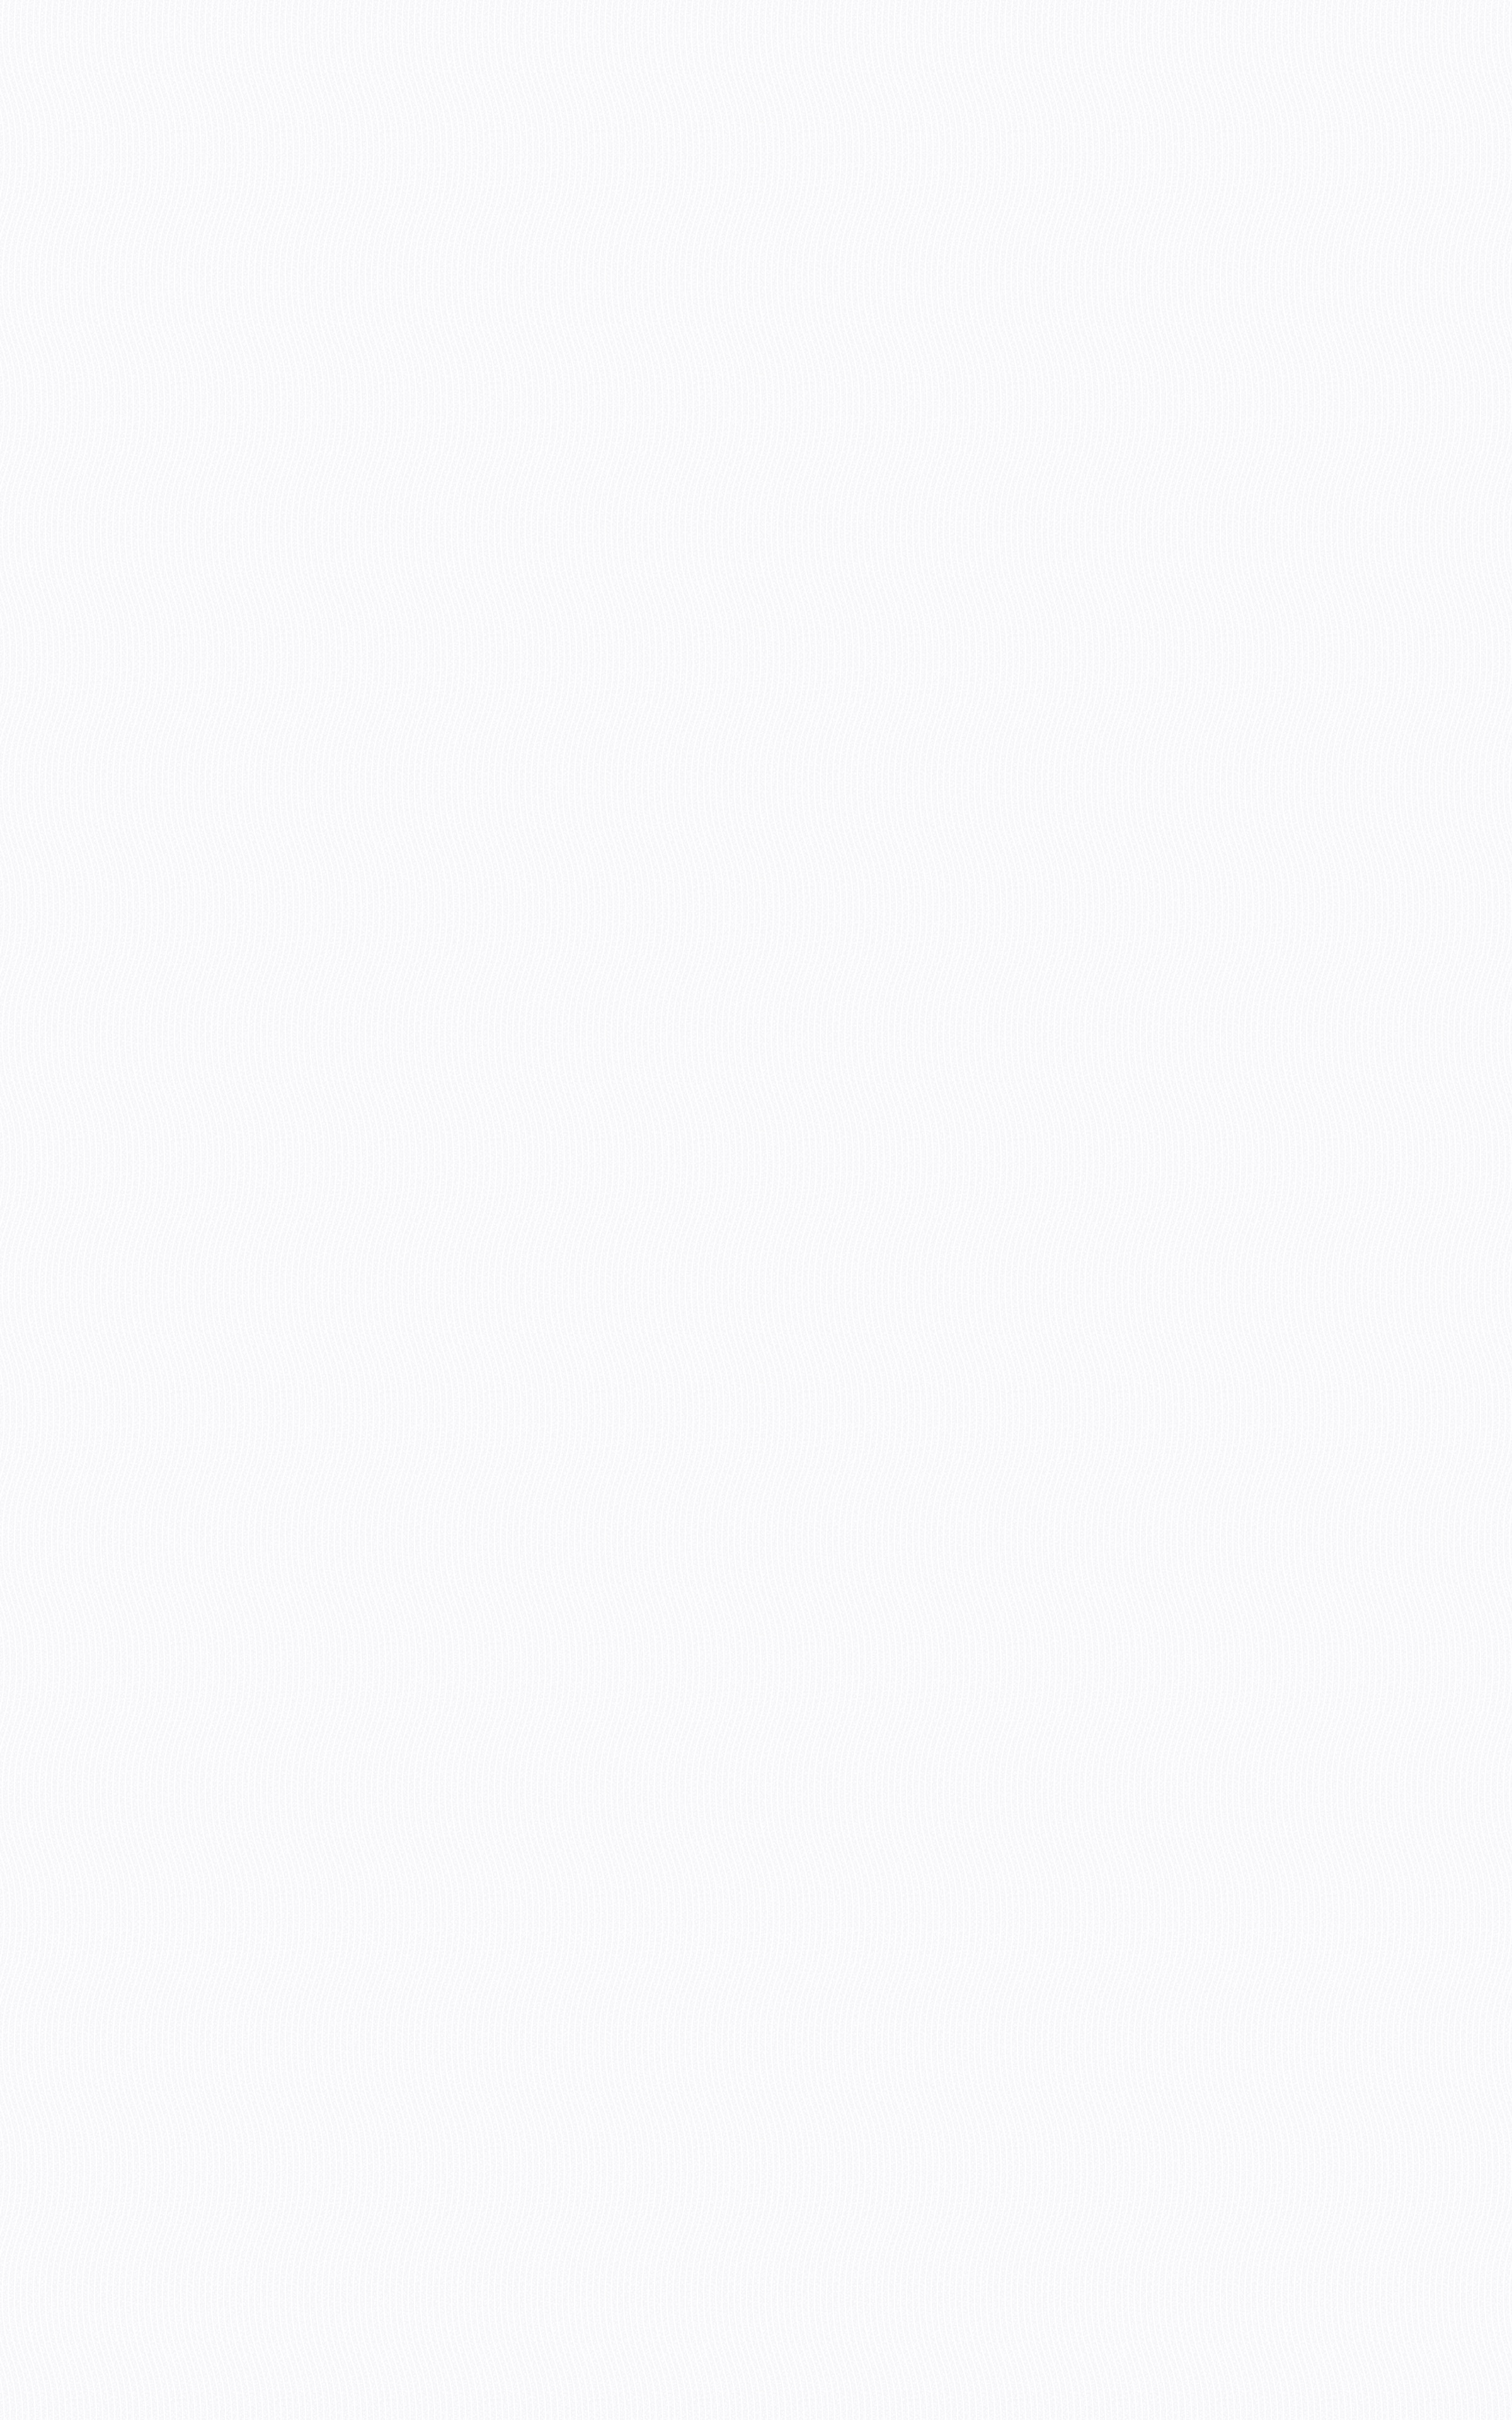
\includegraphics[width=\paperwidth, height=\paperheight, %
%%keepaspectratio]{images/background.jpg}%
%]{images/background.jpg}%
%\vfill
%}}}


\begin{document}
%\AddToShipoutPicture{\BackgroundPic}
\maketitle


\begin{abstract}
Loopring is an open protocol for building decentralized exchanges. Loopring operates as a public set of smart contracts responsible for trade and settlement, with an off-chain group of actors aggregating and communicating orders. The protocol is free, extensible, and serves as a standardized building block for decentralized applications (dApps) that incorporate exchange functionality. Important improvements over current decentralized exchange protocols are the ability for users' orders to be mix-and-matched with other orders, obviating the constraints of two-token trading pairs, drastically improving liquidity, and price improvement possibility. Loopring also employs a robust and unique solution to prevent front-running: the unfair attempt to submit transactions into a block quicker than the original solution provider. Loopring is blockchain agnostic, and deployable on any blockchain with smart contract functionality. At the time of writing, it's operable on Ethereum \cite{buterin2017ethereum} \cite{wood2014ethereum} and Qtum \cite{dai2017smart} with NEO \cite{atterlonn2018distributed} also under construction. Its interoperable standards ensure trustless, decentralized, and anonymous trading. 
\end{abstract}




\section{Introduction\label{sec:introduction}}

With the proliferation of blockchain-based assets, the need to exchange these assets amongst counterparties has significantly increased. As thousands of new tokens are introduced -- including the tokenization of traditional assets - this need is magnified. Whether exchanging for speculative trading motivations, or converting to access networks via their native utility tokens, the ability to exchange one cryptoasset for another is foundational for the larger ecosystem.
 
As such, the trustless exchange of tokens (value) is a compelling use case for blockchain technology. Until now, however, crypto enthusiasts have largely settled for trading tokens on traditional centralized exchanges. The Loopring protocol is needed because, just as Bitcoin \cite{nakamoto2008bitcoin} dutifully pointed out that, in regards to peer-to-peer electronic cash, "the main benefits are lost if a trusted third party is still required to prevent double-spending", so too are the main benefits of decentralized assets lost if they must pass through trusted, gated, centralized exchanges.

Trading decentralized tokens on centralized exchanges doesn't make sense from a philosophical perspective, as it fails to uphold the virtues these decentralized projects espouse. There are also numerous practical risks and limitations in using centralized exchanges which are described below. Decentralized exchanges (DEXs) \cite{schuh2015bitshares} \cite{bancor} \cite{kyber} \cite{warren20170x} have sought to address these issues, and in many cases have succeeded in alleviating security risks. However, there is still vast room for improvement in performance as DEX capability becomes important infrastructure for the new economy. Loopring hopes to provide critical tools for said infrastructure with its open protocol for building DEXs. 

\section{Current Exchange Landscape\label{sec:current_exchange_landscape}}

\subsection{Inadequacies of Centralized Exchanges}
The three primary risks of centralized exchanges are; 1) Lack of security, 2) Lack of transparency, and 3) Lack of liquidity.

\subsubsection{Lack of Security}
Security risks arise from the fact that users must typically surrender control of their private keys (funds) to one centralized entity. This exposes users to the possibility that centralized exchanges fall prey to malicious hackers. The security and hacking risks facing all centralized exchanges are well known \cite{coincheckhack} \cite{mtgox} \cite{mcmillan2014inside}, yet are often accepted as ‘table stakes' for token trading. Centralized exchanges, such as Coinbase and Bittrex, continue to be honeypots for hackers to attack, as their servers control millions of dollars of users' funds. Exchange developers can also make honest, accidental errors with your funds. You are simply not in control of your own tokens when they are deposited at a centralized exchange.

\subsubsection{Lack of Transparency}
Beyond security hacks, a lack of transparency exposes users to the risk of dishonest exchanges acting unfairly. The distinction here is by the exchange operator's malintentions. 

Users are not truly trading their own assets on a centralized exchange, but rather, an IOU - a promissory note that the exchange will redeem your note for your original asset. When tokens are sent to the exchange's wallet, they take custody, and offer an IOU. All trades are then effectively between users' IOUs. To withdraw, you redeem your IOU with the exchange, and get back your tokens to your external wallet address. Throughout this process there is a lack of transparency, and the exchange can shutdown, freeze your account, go bankrupt, etc. It is also possible that they use your assets for other purposes while in custody (such as lending them out to third parties), which makes you susceptible along another attack vector. Lack of transparency can also cost you without total loss of funds, such as in higher trading fees, delays at peak demand, regulatory risk, and your orders being front ran.

\subsubsection{Lack of Liquidity}
From the point of view of exchange operators, fragmented liquidity inhibits entry by new exchanges because of two winner-takes-all scenarios. First, the exchange with the most number of trading pairs available wins, because users find it desirable to conduct all their trades on one exchange. Second, the exchange with the largest order book wins, because of favorable bid-ask spreads for each trading pair. This discourages competition from newcomers because it is difficult for them to build up initial liquidity. As a result, many legacy exchanges command a high market share despite user complaints and even major hacking incidents. It's worth noting that as centralized exchanges win market share, they make themselves an ever-larger hacking target. 

From the point of view of users, fragmented liquidity significantly reduces user experience. In a centralized exchange, users are only able to trade within the exchange's own liquidity pools, against its own order book, and between its supported token pairs. To trade Token A, for Token B, you must go to an exchange that supports both tokens or register at different exchanges, disclosing personal information. You often need to execute preliminary or intermediate trades, usually against BTC or ETH, absorbing bid-ask spreads in the process. Finally, the order books may not be deep enough to complete your trade without material slippage.

The result is disconnected silos of liquidity and a fragmented ecosystem that resembles the legacy financial system, with significant trading volume centralized on few exchanges. The global liquidity promises of blockchains hold no merit within centralized exchanges.

\subsection{Inadequacies of Decentralized Exchanges}
Decentralized exchanges, such as KyberNetwork or EtherDelta, differ from centralized exchanges in that users maintain control of their assets (private keys) by performing trades directly on the underlying blockchain. By leveraging the trustless technology of cryptocurrencies themselves, they successfully mitigate many of the above mentioned risks surrounding security. However, problems persist in regards to performance and structural limitations. 

Liquidity often remains an issue as users must search for counterparties across disparate silos and standards. Fragmented liquidity effects are present if users don't employ consistent standards to interoperate, and if orders are not shared/propagated across a wide network. 

Furthermore, since trades are performed on chain, DEXs often inherit the limitations of the underlying blockchain, namely: scalability, delays in execution (mining), and costly modifications to orders. Thus, blockchain order books do not scale well, as executing code on the blockchain incurs a cost (gas), making multiple order-cancel cadences prohibitively expensive. 

Finally, because blockchain order books are public, the transaction to place an order is visible by miners as it awaits being mined into the next block, and placed into an order book. This delay exposes the user to the risk of being front run and having the price move against him.

\subsection{Hybrid Solutions}
For the above reasons, purely blockchain-based exchanges have limitations that make them uncompetitive with centralized exchanges. There is a tradeoff between on-chain inherent trustlessness, and centralized exchange speed and order flexibility. Protocols such as Loopring and 0x \cite{warren20170x} extend a solution of on-chain settlement with off-chain order relay. These solutions revolve around open smart contracts, but navigate scalability limitations by performing several functions off-chain, and giving nodes flexibility in fulfilling critical roles for the network. While Loopring admires protocols such as 0x, as we demonstrate throughout the paper, we propose meaningful differences in our approach to a hybrid solution.


\section{Loopring Protocol\label{sec:loopring_protocol}}
Loopring is not a DEX, but a protocol for building DEXs on multiple blockchains. We disassemble the component parts of a traditional exchange and offer a set of public smart contracts and decentralized actors in its place. The roles in the network include wallets, relays, liquidity-sharing consortium blockchains, order book browsers, ring-miners, and asset tokenization services. Before defining each, we should first understand what a Loopring compliant order looks like. 

\subsection{Order Ring}
Loopring orders are expressed in what we call a Unidirectional Order Model (UDOM \cite{coinport2014udom}). UDOM expresses orders as token exchange requests - amountS/amountB - instead of bids and asks. Since every order is just an exchange rate between two tokens, a powerful feature of the protocol is the mixing and matching of multiple orders in circular trade. By using up to 10 orders instead of a single trading pair, there is a dramatic increase in liquidity and potential for price improvement. 

Each order's token to sell is another order's token to buy. It creates a loop that allows each order to exchange their desired tokens without requiring an opposing order for its pair. Traditional order pair trades can, of course, still be executed, in what is essentially a special case of an Order Ring. 


\begin{definition}[Order Ring] Let $C_{0}$, $C_{1}$, $\cdots$, $C_{n-1}$ be $n$ different kinds of token, $O_{0\rightarrow 1}$, $\cdots$, $O_{i\rightarrow i\oplus 1}$, $\cdots$, $O_{n-1 \rightarrow 0}$ be $n$ orders. Those orders can form a ring for trading:
$$O_{0\rightarrow 1} \rightarrow \cdots \rightarrow O_{i\rightarrow i\oplus 1} \rightarrow \cdots \rightarrow O_{n-1\rightarrow 0} \text{, }$$
where $n$ is the length of the ring, and $i\oplus 1 \equiv i+1 \mod n$.
\end{definition}

An order ring is valid when all component transactions can be executed at an exchange rate equal to or better than the original rate specified by the user. To verify ring validity, Loopring protocol smart contract (protocol) must receive Order Rings from miners where the product of the original exchange rates of all orders is equal to or greater than 1. (further calculations in section 4).

Every order has two basic elements: two assets offered for trading and an exchange rate. The price is the exchange rate with one of the assets fixed as parameter. Let assume Alice and Bob want to trade their tokens A and B. Alice has 15 tokens A and she wants 4 tokens B for them; Bob has 10 tokens B  and he wants 30 tokens A for them.

Who is buying and who is selling? This depends only on the asset we fix to give price quotations. If token A is the reference, then Alice is buying tokens B for ${15 \over 4} = 3.75$ XTA, while Bob is selling 10 tokens B for ${30 \over 10} = 3.00$ XTA. In the case of fixing token B as reference we say that Alice is selling 15 tokens A for ${4\over 15}=0.26666667$ XTB and Bob is buying 10 tokens A for ${10 \over 30}=0.33333334$ XTB. Hence, who's the buyer or seller is purely arbitrary.

In the first situation Alice is willing to pay a higher price than the price Bob is selling his tokens for, in the second situation Bob is willing to pay a higher price than the price Alice is selling her tokens for. It is clear that a trade is possible whenever the buyer is willing to pay an equal or higher price than the selling price, no matter how we fix the prices. If we recall our basic arithmetic we learned in school we can verify easily that:

\begin{equation}
{{15\over 4} \over {30\over 10}} = {3.75 \over 3.00}	= {0.33333334 \over 0.26666667} = {{10 \over 30} \over {4 \over 15}} = {15 \over 4} \cdot {10 \over 30} = {150 \over 120} = 1.25 > 1
\end{equation}

In this article, we reference this as the Uni-Directional Order Model, or UDOM for short. See \ref{anatomy} for more details about Loopring's orders.


\section{Ecosystem Participants}
The following ecosystem participants jointly provide all functionalities a centralized exchange has to offer. 

\begin{itemize}

\item \textbf{Wallets}: A common wallet service or interface that gives you access to your tokens and a way to send orders to the Loopring network. Wallets will be incentivized to produce orders by sharing fees (see section 5.1).

\item \textbf{Relays / Ring Miners}: Relays are nodes that form a decentralized network for order propagation. They maintain public order books and trade history and broadcast new orders to other relays via any arbitrary off-chain medium. Ring-mining is a feature of relays. It is computational heavy and is done completely off-chain. Ring-mining produces Order Rings: rings of between 2 and 10 tokens created by stitching together disparate orders. Relays are free in how they choose to communicate with one another (or not). 

\item \textbf{Consortium Liquidity Sharing Blockchain}: TODO(daniel)

\item \textbf{Loopring Protocol Smart Contracts}: A set of public and free smart contracts that checks Order Rings received from miners, does token transfers on behalf of users, incentivizes miners/wallets, and emits events. Relays/order browsers listen to these events to keep their order books and trade history up to date.

\item \textbf{Asset Tokenization Services}: A bridge between assets that cannot be directly traded on Loopring. They are centralized services run by trustworthy companies or organizations. A user could deposit his assets (real, fiat or tokens from other chains) and get tokens issued. By returning these tokens the user gets back his deposit. Loopring is not a cross-chain exchange protocol, but Asset Tokenization Services make it possible to trade Ethereum ERC20 \cite{ERC20} tokens with physical assets as well as assets on other blockchains. 

\end{itemize}


\section{Exchange Process}
\begin{enumerate} 

\item \textbf{Order Initiation \& ERC20 Authorization}: A user wants to exchange X amount of TokenA for Y amount of TokenB. The current rate and order book for this pair can be found on multiple sources provided by relays or other interfaces hooked up to the network, such as order book browsers (4). The user places an order through a wallet interface. An amount of LRx can be added to the order as a fee for miners; higher LRx fee means a better chance to be processed earlier by miners. The wallet authorizes the LSC to handle X amount of TokenA the user wants to sell, but does not lock the user's tokens, who remains free to move them while the order is being processed.

\item \textbf{Send order to the network}: Once the authorization is made, the order's data is signed with the private key of the sender. Then, the wallet sends the order along with its signature to one or more nodes (relays) in the network.
\item \textbf{Relay broadcast}: On the reception of the order, relays update their public order book and broadcast the order to other relays/ring miners. The protocol doesn't require order books to be built in a certain way, for example, first-come-first-serve. Instead, relays have the power to make their own design decisions to build their own order books.
\item \textbf{Ring-mining (order matching)}: Ring Miners receive the order and add it to their order book. Each miner tries to fill it fully or partially at the given exchange rate or better by ring-matching it with multiple other orders. Ring-matching is the main reason why the protocol is able to provide high liquidity over any pair. If the executed rate is better than what the user asked for, the savings (margin) are shared amongst all orders in the ring. As a reward (fee), the miner can choose between claiming the Margin Split and giving back the LRx to the user, or just keeping the LRx fee.
\item \textbf{Verification \& Settlement}: The ring is received by the Loopring Smart Contract. It makes multiple checks to verify the miner's supplied data and determines if the ring can be settled fully or partially (depending on the fill rate of orders in the ring and the tokens in the users' wallets). If all checks are successful, the contract automatically makes the token transfers to the users and pays the miner's fees at the same time. If the sender's balance as determined by the LSC are insufficient, it will be considered scaled-down. A scaled-down order is not the same as a cancelled order: a scaled-down order will automatically scale up to its original size if sufficient funds are deposited to its address, while cancellation is a one way manual operation and can't be reversed.

\end{enumerate}

\section{Business Model Flexibility}
It's important to note that Loopring's open standard allows participants significant flexibility in how they conduct ‘business'. Actors with novel business models are free to implement them and provide value for their users, earning LRx fees on volume in the process.
\subsection{Order Book}
Relays can design their order books in any number of ways to display and match users' trades. A first implementation of our own order book follows an OTC model, where limit orders are ‘ranked' or positioned based on price alone. Timestamps of orders, in other words, have no bearing on the order book. However, a relay is free to design their order book in such a way as to emulate a typical centralized exchange's matching engine, where orders are ranked by price, but with a timestamp respecting filter as well. If a relay was inclined to offer this type of order book, they can own/integrate with a wallet, and have those wallet orders sent solely to the single relay, who would then be able to match orders based on time. Any such configuration is possible. 

\subsection{Liquidity Sharing}
Relays are similarly free to design how they share liquidity and orders with one another. Our consortium blockchain is but one solution to accomplish this, and the ecosystem is free to network and communicate as they wish. Besides joining a consortium blockchain, they can build and manage their own, creating rules/incentives as they see fit. Relays can also work solo, as seen in the time-sensitive wallet implementation above. Of course, there are clear advantages in communicating with other relays in pursuit of network effects, however, different business models could merit peculiar sharing designs. 



\section{Protocol Specification}

\subsection{Anatomy of an Order\label{anatomy}}
An order is a pack of data that describes the intent of the user's trade. A Loopring order is defined using the Uni-Directional Order Model, or UDOM, as follows:

\begin{verbatim}
  message Order {
    address protocol;
    address owner;
    address tokenS;
    address tokenB;
    uint256 amountS;
    uint256 amountB;
    unit256 lrcFee
    unit256 validSince;             // Seconds since epoch
    unit256 validUntil;             // Seconds since epoch
    uint8   marginSplitPercentage;  // In the rage of [1-100]
    bool    buyNoMoreThanAmountB;
    uint256 walletId;
    address authAddr; // Dual-Authoring address
    uint8   v;        // Part of the signature
    bytes32 r;        // Part of the signature
    bytes32 s;        // Part of the signature
    string  _authKey; // Dual-Authoring private key,
                      // it is not used for calculating order's hash.
  }
\end{verbatim}
To ensure the origin of the order, it is signed against the hash of its parameters, excluding $\_authAddr$, with the user's private key. The $\_authAddr$ parameter is used for signing  order rings that this order is part of, which prevents front-running. Please reference \ref{dual_authoring} for more details. The signature is represented by the $v$, $r$, and $s$ fields, and is sent alongside the order parameters over the network. This guarantees the order stays immutable during its whole lifetime. Even though the order never changes, the protocol can still compute its current state based on the balance of its address along with other variables.


UDOM doesn't include a price (which must be a floating-point number by nature), but, instead uses the term $rate$, which is expressed as $amountS \over amountB$. The rate is not a floating-point number but an expression that will only be evaluated with other unsigned integers on demand, to keep all intermediate results as unsigned integers and increase calculation accuracy. 

When a miner ring-matches orders, it's possible that a better rate will be executable, allowing you to get more $tokenB$ than the $amountB$ you specified. However, if $buyNoMoreThanAmountB$ is set to $true$, the protocol ensures you receive exactly $amountB$ of $tokenB$. Thus, UDOM's $buyNoMoreThanTokenB$ parameter determines when an order is considered completely filled. $buyNoMoreThanTokenB$ applies a cap on either $amountS$ or $amountB$, and allows users to express more granular trade intentions than traditional buy/sell orders. 

If we use

\begin{equation}
	Order(amountS, tokenS, amountB, tokenB, buyNoMoreThanTokenB)
\end{equation}

to represent a order in a simplified form, then for ETH/USD markets on a traditional exchange, traditional buy-sell modeling can express the 1st and the 3rd order below, but not the other two:

\begin{enumerate}
	\item User wants to sell 10 ETH at price 300 USD/ETH. This order can expressed as $Order(10, ETH, 3000, USD, false)$.
	\item User wants to sell ETH at price 300 USD/ETH to get 3000 USD. This order can expressed as $Order(10, ETH, 3000, USD, true)$.
	\item User wants to buy 10 ETH at price 300 USD/ETH, This order can expressed as $Order(3000, USD, 10, ETH, true)$.
	\item User wants to spend 3000 USD to buy as many ETH as possible at price 300 USD/ETH, This order can expressed as $Order(3000, USD, 10, ETH, false)$.
\end{enumerate}





\subsection{Ring Verification}

LSC does not perform exchange rate or amount calculations, but must receive and verify what the miner supplied for these values. This is done by miners for two main reasons: solidity does not have support for floating point maths, especially pow(x, 1/n), and it is desirable for the computation to be made off-chain to save gas.

\subsubsection{Sub-Loop Checking}
This step prevents arbitrageurs from unfairly realizing all the margin in a ring by implementing new orders within it. Essentially, once a valid ring is found by a miner, it could be tempted to add other orders to the ring to fully absorb the users' margin (rate discounts). This is zero-risk, zero-value add to the network, and is considered unfair conduct by the miner. To prevent this, Loopring requires that a valid loop cannot contain a sub-loop. To check this, LSC ensure a token cannot be in a buy or sell position twice. In the above diagram we can see that ARK is a sell token twice, and a buy token twice, which would be disallowed. 

\subsubsection{Fill Rate Checking}
The exchange rate calculations in the ring are made by miners for reasons stated above. It is the LSC that must verify they're correct. First, it verifies that the buy rate the miner can execute for each order is at least equal to or less than the original buy rate set by the user. This ensures the user gets at least the exchange rate they asked for or better on the transaction. Once the exchange rates are confirmed, LSC makes sure that all the margins (discounts) are the same percentage for every order, to ensure fairness.

According to Loopring protocol, each order in the ring would share the same rate (price) discount. For instance, if the discounted rate is $\gamma$, then the price for each order will be:
$r_{0\rightarrow 1} \cdot (1-\gamma)$, $r_{1\rightarrow 2} \cdot (1-\gamma)$, $r_{2 \rightarrow 0} \cdot (1-\gamma)$, and satisfied: 
\begin{equation}
r_{0\rightarrow 1} \cdot (1-\gamma)\cdot r_{1\rightarrow 2} \cdot (1-\gamma) \cdot r_{2 \rightarrow 0} \cdot (1-\gamma) = 1
\end{equation}
We can find out: 
\begin{equation*}
\gamma = 1- \frac{1}{\sqrt[3]{r_{0\rightarrow 1} \cdot r_{1\rightarrow 2} \cdot r_{2\rightarrow 0}}}\text{.}
\end{equation*}
In the other circumstance, if transaction cross $n$ orders, the \texttt{discount} is: 
\begin{equation*}
\gamma = 1- \frac{1}{\sqrt[n]{\prod_{i=0}^{n-1} r^i}} \text{,}
\end{equation*}
where $r^i$ is the order turnover rate of $i$-th order. Obviously, only when the discount rate is $\gamma \ge 0$, these orders can be filled; and the $i$-th order's $O^i$ actual exchange rate $\hat{r^i} = r^i \cdot (1-\gamma)$, $\hat{r^i}\le r^i$.

\subsubsection{Fill Tracking \& Cancellation}
A user can partially or fully cancel an order by sending a special transaction to the LSC, containing the details about the order and the amounts to cancel. The LSC takes that into account, stores the amounts to cancel, and emits an OrderCancelled event to the network. The LSC keeps track of fill and cancellation amounts by storing their values using the order's hash as an identifier. This data is publicly accessible and OrderCancelled / OrderFilled events are emitted when it changes. Tracking these values is critical for the LSC during the ring settlement step.


\subsubsection{Order Scaling}
Orders are scaled according to the history of filled and cancelled amounts and the current balance of the senders' accounts. The process finds the order with the smallest amount to be filled according to the above characteristics and uses it as a reference for scaling all transactions in the ring.


Finding the lowest value order can help to figure out the fill volume for each order. For instance, if the $i$-th order is the lowest value order, then the number of tokens sold from each order $\hat{s}$ and number of tokens purchased $\hat{b}$ from each order can be calculated as:

\[
\begin{split}
&\hat{s}^{i}=\overline{s}_i\text{, } \hat{b}^{i}=\hat{s}^{i}/ \hat{r}^i\text{, }\text{;}\\
&\hat{s}^{i\oplus 1}=\hat{b}^i\text{, } \hat{b}^{i\oplus 1}=\hat{s}^{i\oplus 1}/ \hat{r}^{i\oplus 1}\text{;}\\
&\hat{s}^{i\oplus 2}=\hat{b}^{i\oplus 1}\text{, } \hat{b}^{i\oplus 2}=\hat{s}^{i\oplus 2}/ \hat{r}^{i\oplus 2}\text{;}\\
& ...
%\text{.}
\end{split}
\]
where $\overline{s}_i$ is the the balance left after orders are partially filled.

During implementation we can safely assume any order in the ring to have the lowest value, then iterate through the ring at most twice to calculate each orders' fill volume. 

Example: If the smallest amount to be filled compared to the original order is 5\%, all the transactions in the ring are scaled down to 5\%. Once the transactions are completed, the order that was considered to have the smallest amount remaining to be filled should be completely filled.

\subsection{Ring Settlement}

If the Order Ring fulfills all the previous checks, the ring can be closed, and transactions can be made. This means that all the $n$ orders $O$ form a closed ring of orders, connected as in the figure below:

[TODO: DIAGRAM]

To make the transactions, the LSC uses the $TokenTransferDelegate$ smart contract. The introduction of such a delegate makes upgrading the protocol smart contract easier as all orders only need to authorize this delegate instead of different versions of the protocol.

For each order in the ring, a payment of $tokenS$ is made to the following order. Then the miner's fee is paid depending on the fee model chosen by the miner. An $OrderFilled$ event is then emitted. Finally, once all the transaction are made, a $RingMined$ event is emitted.

\subsubsection{Emitted Events}

The protocol emits events that allow relays, order browsers, and other actors to receive order book updates as efficiently as possible. The emitted events are:

\begin{itemize}
	\item \textbf{OrderCancelled}: a specific order has been cancelled.
	\item \textbf{OrdersCancelled}: all orders of a trading pair for an owning address have been cancelled.
	\item \textbf{AllOrdersCancelled}: all orders of all trading pairs for an owning address have been cancelled.	
	\item \textbf{RingMined}: A ring has been settled successfully. This event contains data related to each inner-ring token transfer.
\end{itemize}


\section{LRx Token}
LRx is our generalized token notation. LRC is the Loopring token on Ethereum, LRQ on Qtum, and LRN on NEO. More LRx will be introduced in future as Loopring is deployed on other public blockchains.

\subsection{Fee Model} 
When a user creates an order, they specify an amount of LRx to be paid to the miner as a fee, in conjunction with a percentage of the margin made on the order that the miner can claim. This is called the margin split. The decision of which one to choose is left to the miner.

A representation of the margin split:

[TODO: daniel wang]

If the margin on the ring is too small, a miner will choose the LRx fee. On the contrary, if the margin is substantial enough for the resulting margin split to be worth more than the LRx fee, they will choose the margin split. There is another proviso, however: when the miner chooses the margin split, they must pay the user (order creator) a fee, which is equal to the LRx the user would have paid to the miner as a fee. This increases the threshold of where the miner will choose the margin split to twice the LRx fee of the order, increasing the propensity of the LRx fee choice. This allows miners to get a constant income on low margin rings with for the tradeoff of getting less income on higher margin rings. Our fee model is based on the expectation that as the market grows and matures, there will be fewer high margin rings, thus necessitating LRx fees as incentive.
We end up with the following graph:

[TODO: daniel wang]

where $f$ is the LRx fee, $x$ is the margin split, $y$ is the miner's income.

If $f$ is the LRx fee and $x$ the margin split, then the miner's income $y$ is $y=max(f, x-f)$ and we get the blue line; if the LRx fee for the order is $0$, the equation is $y=max(0, x - 0)$ that simplifies to $y=x$ and we get the orange line.

The consequences are:  
\begin{enumerate}
	\item If the margin split is 0, the miners will choose the flat LRx fee and are still incentivized. 
	\item If the LRx fee is 0, the orange line results and the income is based on a general linear model.
	\item When the margin split income > 2*(LRx fee), the miner chooses the margin split.
\end{enumerate}

It should be noted that if the LRx fee is non-zero, no matter which option the miner chooses, there will always be a transfer of LRx between the miner and the order's sender. Either the miner earns the LRx fee, or pays the LRx fee back to the sender to take the margin split.

Ring miners will share a certain percentage of fees with wallets. When a user places an order through a wallet and it is filled, the wallet is rewarded with a portion of the fees or margin split. Wallets represent a primary target for protocol integration as they have the user base, but little source of income. 

\subsection{Decentralized Governance}
LRx tokens are used to align the financial incentives of the various participants in the network. Such alignment is necessary for broad adoption of the protocol, whose success rests largely on improving liquidity in a robust decentralized ecosystem.

LRx tokens will be used to effectuate protocol updates through decentralized governance. Smart contract upgrades will be voted on by token holders to dissuade rogue forks from potentially siphoning off liquidity through incompatibility. Upgradeability is crucial to the protocol's success as it must adapt to market demands, and the changing underlying blockchains.

\section{Fraud and Attack Protections}

\subsection{Dual-Authoring: Front-running Prevention}

In decentralized exchanges, front-running is when someone tries to copy another node's ring solution, and have it mined before the original transaction that is in the pending transaction pool (mempool). This can be achieved by specifying a higher transaction fee (gas price). The major scheme of front-running in Loopring (and any protocol for order-matching) are order-filch: when a front-runner steals one or more orders from a pending ring settlement transaction; and Ring-filch: when a front-runner steals the entire ring from the pending transaction.

When a submitRing transaction is not confirmed and still in the pending transaction pool, anyone can easily spot such a transaction and replace $miner\_address$ with their own address (the filcher\_address) , then they can re-sign the payload with filcher\_address to replace the ring's signature. The fincher can set a higher gas price and submit a new transaction hoping block miners will pick his new transaction into the next block instead of the original submitRing transaction.
Previous solutions to this problem had important downsides (v1.1): it requires more transactions and thus cost miners more gas; and it takes at least twice the blocks to settle a ring.  Our new solution involves the mechanism of setting up two levels of authorization for orders - one for settlement, and one for mining.
How it works:

\begin{enumerate}

	\item For each order, the wallet software will generate a random public- key/private-key pair, and put the key pair into the order's JSON snippet. (An alternative is to use the address derived from the public-key instead of the public-key itself to reduce byte size. We use $authAddr$ to represent such an address, and $\_authKey$ to represent $authAddr$'s matching private-key).

	\item All fields in the order except $\_authKey$ is signed using the $owner$ address's private-key (not $\_authKey$) as shown in the image below.

	\item The wallet will send the order, together with the $\_authKey$ to miners (relays) for matching.The miner will verify that $\_authKey$ and $authAddr$ are correctly paired and the order's signature is valid with respect to owner\_address.

	\item When a ring is identified, the miner will use each order's $\_authKey$ to sign the ring's hash, $miner\_address$, and all the mining parameters. In the example below, the ring contains 3 orders, therefore there will be 3 signatures by the 3 $\_authKey$s. We call these signatures the $auth\_signature$s. The miner also needs to sign the ring's hash together with all mining parameters using $miner\_address$'s private-key.

	\item The miner calls the submitRing function with all the parameters, as well as the 3 extra $auth\_signature$s. Notice that$\_authKey$s are NOT part of the on-chain transaction and thus remain unknown to people other than the relay itself, as shown in the image below.

	\item The Loopring Protocol will now verify each $auth\_signature$ against the corresponding $authAddr$ of each order, and reject the ring if any $auth\_signature$ is invalid.
 
\end{enumerate}
[TODO: daniel wang]


The result it that now:

\begin{itemize}

	\item  The order’s signature (by the private-key of the $owner\_address$) guarantees the order cannot be modified, including the $authAddr$.
	\item  The miner’s signature (by the private-key of the $miner\_address$) guarantees nobody can use his identity to mine a ring.
	\item  The $auth\_signature$s guarantees the entire ring cannot be modified, including $miner\_address$. And since ring-filchers do not have access to $\_authKey$s, they cannot re-generate a new set of $auth\_signature$s thus are unable to generate a filch transaction.

\end{itemize}

Dual Authoring prevents ring-filch and order-filch while still ensuring the settlement of rings can be done in one single transaction. In addition, Dual Authoring opens doors for relays to share orders in two ways: non-matchable sharing and matchable sharing. Loopring operates an OTC model, meaning that orders’ timestamps are totally ignored. This implies that front-running a trade has no impact on the actual price of that trade .  Loopring only supports limit-price orders.

\section{Other Attacks}

\subsection{Denial of Service}
Loopring allows nodes (relayers) to selectively handle orders by setting their own criteria - which they may hide or reveal. By empowering relayers to dictate how they manage orders, we do not see denial of service as a form of unethical behaviour.

\subsection{Sybil Attack}
A user could send a large amount of tiny orders to attack the Loopring nodes. However, since we allow nodes to reject orders based on their own criteria, most of these orders will be rejected because they do not yield satisfying profit when matched. Thus, a massive tiny order attack is not feasible.

\subsection{Insufficient Balance}
Malicious users may sign and spread out orders whose value inside the order is non-zero but whose address actually has zero balance. Nodes could monitor and notice that some orders actual balance is zero, update these orders states accordingly and then discard them.
Nodes have to spend time to update the status of an order, but can also choose to minimize the effort by, for example, blacklisting addresses and drop related orders.


\section{Summary}
Money, as an intermediate commodity, is used to facilitate barter exchange and solve the double coincidence of wants problem \cite{unenumerated2006}. Similarly, Loopring protocol aims to dispense of our dependencies on coincidence of wants in trading pairs. With ring matching, double coincidence of wants is no longer required before a trade could be consummated. This is profound for how society and capital markets transfer value with tokens, traditional assets, and beyond.

\begin{itemize}
	\item Off-chain order management and on-chain settlement = no sacrifice in performance for security.
Network is maintained by a self-motivated group of relays who have flexibility in running their order books.
	\item Greater liquidity due to more counterparties available through order sharing, and increasing probability that any counterparty can be a useful trading partner due to multi-party trades.
	\item Orders can be propagated through arbitrary communication mediums, and liquidity siloes can be connected.
	\item Free, public smart contracts enable any dApp to build or interact with our protocol.
	\item Standardization among operators allows for network effects, deeper liquidity and an improved end user experience.
	\item Reduced barriers to entry for market makers mean lower costs for nodes joining the network and end users.
	\item Anonymous trading directly from users’ wallets.
\end{itemize}

\section{Acknowledgements}
We would like to express our gratitude to our mentors, advisers and to the many people in the community that have been so welcoming and generous with their knowledge. In particular, we would like to thank Shuo Bai (from ChinaLedger); Professor Haibin Kan; Alex Cheng, Hongfei Da; Yin Cao; Xiaochuan Wu; Zhen Wang, Wei Yu, Nian Duan, Jun Xiao, Jiang Qian, Jiangxu Xiang, Yipeng Guo, Dahai Li, Kelvin Long, Huaxia Xia, Jun Ma, and Encephalo Path for reviewing and providing feedback on this project. We also welcome more feedback from the community.



\bibliography{whitepaper2}
\bibliographystyle{unsrt}

\newpage

\begin{figure}[h]
\centering
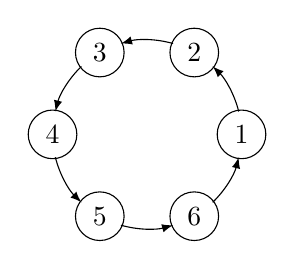
\begin{tikzpicture}

\def \n {6}
\def \radius {1.2cm}
\def \margin {14} % margin in angles, depends on the radius

\foreach \s in {1,...,\n}
{
  \node[draw, circle] at ({360/\n * (\s - 1)}:\radius) {$\s$};
  \draw[->, >=latex] ({360/\n * (\s - 1)+\margin}:\radius) 
    arc ({360/\n * (\s - 1)+\margin}:{360/\n * (\s)-\margin}:\radius);
}


\end{tikzpicture}
\caption{FOSS in Chrome influences industry structure by increasing competition}
\label{fig:6forces}
\end{figure}



\begin{figure}[h]
\centering
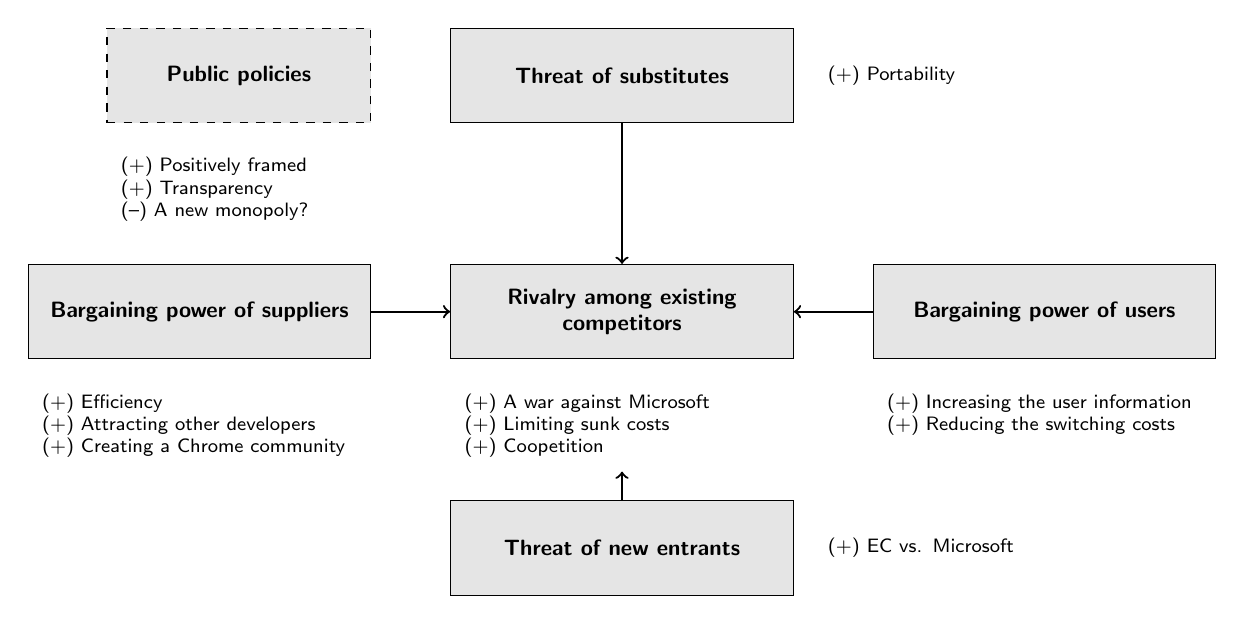
\begin{tikzpicture}
[node distance = 1cm, auto,font=\footnotesize,
% STYLES
every node/.style={node distance=3cm},
% The comment style is used to describe the characteristics of each force
comment/.style={rectangle, inner sep= 5pt, text width=4cm, node distance=0.25cm, font=\scriptsize\sffamily},
% The force style is used to draw the forces' name
force/.style={rectangle, draw, fill=black!10, inner sep=5pt, text width=4cm, text badly centered, minimum height=1.2cm, font=\bfseries\footnotesize\sffamily}] 

% Draw forces
\node [force] (rivalry) {Rivalry among existing competitors};
\node [force, above of=rivalry] (substitutes) {Threat of substitutes};
\node [force, text width=3cm, dashed, left=1cm of substitutes] (state) {Public policies};
\node [force, left=1cm of rivalry] (suppliers) {Bargaining power of suppliers};
\node [force, right=1cm of rivalry] (users) {Bargaining power of users};
\node [force, below of=rivalry] (entrants) {Threat of new entrants};

%%%%%%%%%%%%%%%
% Change data from here

% RIVALRY
\node [comment, below=0.25 of rivalry] (comment-rivalry) {(+) A war against Microsoft\\
(+) Limiting sunk costs\\
(+) Coopetition};

% SUPPLIERS
\node [comment, below=0.25cm of suppliers] {(+) Efficiency\\
(+) Attracting other developers\\
(+) Creating a Chrome community};

% SUBSTITUTES
\node [comment, right=0.25 of substitutes] {(+) Portability};

% USERS
\node [comment, below=0.25 of users] {(+) Increasing the user information\\
(+) Reducing the switching costs};

% NEW ENTRANTS
\node [comment, right=0.25 of entrants] {(+) EC vs. Microsoft};

% PUBLIC POLICIES
\node [comment, text width=3cm, below=0.25 of state] {(+) Positively framed\\
(+) Transparency\\
(--) A new monopoly?};

%%%%%%%%%%%%%%%%

% Draw the links between forces
\path[->,thick] 
(substitutes) edge (rivalry)
(suppliers) edge (rivalry)
(users) edge (rivalry)
(entrants) edge (comment-rivalry);

\end{tikzpicture} 
\caption{FOSS in Chrome influences industry structure by increasing competition}
\label{fig:6forces}
\end{figure}

\begin{figure}[h]
\centering
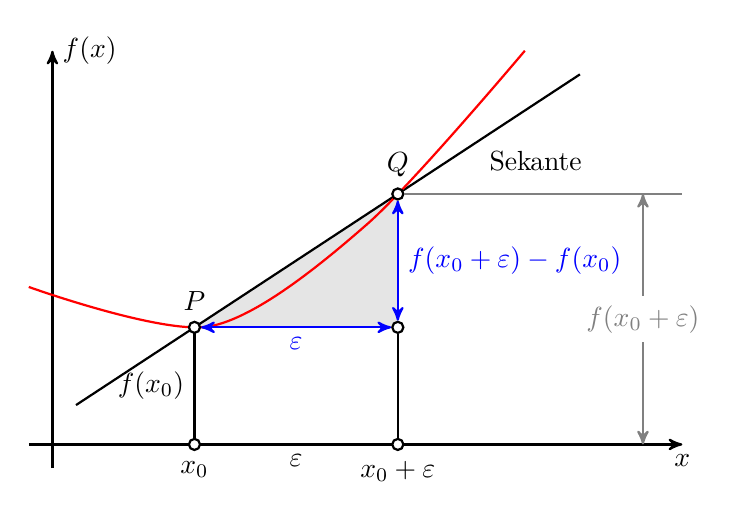
\begin{tikzpicture}[
    thick,
    >=stealth',
    dot/.style = {
      draw,
      fill = white,
      circle,
      inner sep = 0pt,
      minimum size = 4pt
    }
  ]
  \coordinate (O) at (0,0);
  \draw[->] (-0.3,0) -- (8,0) coordinate[label = {below:$x$}] (xmax);
  \draw[->] (0,-0.3) -- (0,5) coordinate[label = {right:$f(x)$}] (ymax);
  \path[name path=x] (0.3,0.5) -- (6.7,4.7);
  \path[name path=y] plot[smooth] coordinates {(-0.3,2) (2,1.5) (4,2.8) (6,5)};
  \scope[name intersections = {of = x and y, name = i}]
    \fill[gray!20] (i-1) -- (i-2 |- i-1) -- (i-2) -- cycle;
    \draw      (0.3,0.5) -- (6.7,4.7) node[pos=0.8, below right] {Sekante};
    \draw[red] plot[smooth] coordinates {(-0.3,2) (2,1.5) (4,2.8) (6,5)};
    \draw (i-1) node[dot, label = {above:$P$}] (i-1) {} -- node[left]
      {$f(x_0)$} (i-1 |- O) node[dot, label = {below:$x_0$}] {};
    \path (i-2) node[dot, label = {above:$Q$}] (i-2) {} -- (i-2 |- i-1)
      node[dot] (i-12) {};
    \draw           (i-12) -- (i-12 |- O) node[dot,
                              label = {below:$x_0 + \varepsilon$}] {};
    \draw[blue, <->] (i-2) -- node[right] {$f(x_0 + \varepsilon) - f(x_0)$}
                              (i-12);
    \draw[blue, <->] (i-1) -- node[below] {$\varepsilon$} (i-12);
    \path       (i-1 |- O) -- node[below] {$\varepsilon$} (i-2 |- O);
    \draw[gray]      (i-2) -- (i-2 -| xmax);
    \draw[gray, <->] ([xshift = -0.5cm]i-2 -| xmax) -- node[fill = white]
      {$f(x_0 + \varepsilon)$}  ([xshift = -0.5cm]xmax);
  \endscope
\end{tikzpicture}
\caption{FOSS in Chrome influences industry structure by increasing competition}
\label{fig:6forces}
\end{figure}




\begin{figure}[h]
\centering
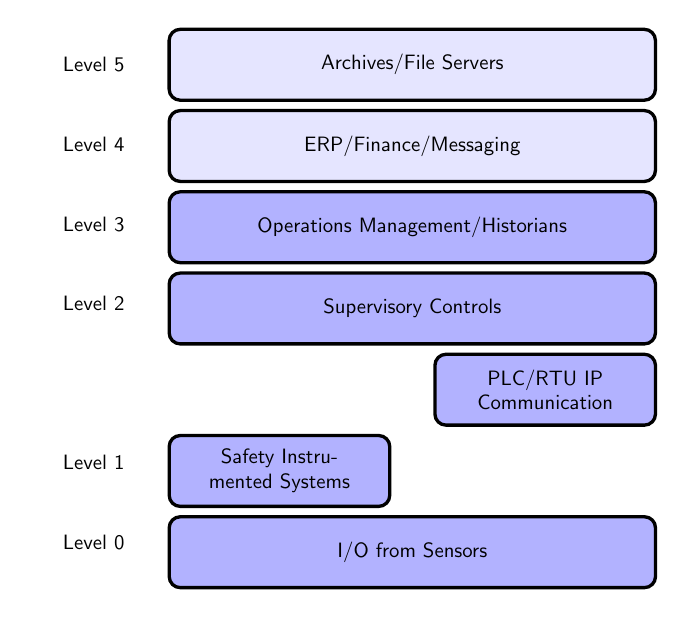
\begin{tikzpicture}[
	scale=0.75,
	start chain=1 going below, 
	start chain=2 going right,
	node distance=1mm,
	desc/.style={
		scale=0.75,
		on chain=2,
		rectangle,
		rounded corners,
		draw=black, 
		very thick,
		text centered,
		text width=8cm,
		minimum height=12mm,
		fill=blue!30
		},
	it/.style={
		fill=blue!10
	},
	level/.style={
		scale=0.75,
		on chain=1,
		minimum height=12mm,
		text width=2cm,
		text centered
	},
	every node/.style={font=\sffamily}
]

% Levels
\node [level] (Level 5) {Level 5};
\node [level] (Level 4) {Level 4};
\node [level] (Level 3) {Level 3};
\node [level] (Level 2) {Level 2};
\node [level] (Level 1.5) { };
\node [level] (Level 1) {Level 1};
\node [level] (Level 0) {Level 0};

% Descriptions
\chainin (Level 5); % Start right of Level 5
% IT levels
\node [desc, it] (Archives) {Archives/File Servers};
\node [desc, it, continue chain=going below] (ERP) {ERP/Finance/Messaging};
% ICS levels
\node [desc] (Operations) {Operations Management/Historians};
\node [desc] (Supervisory) {Supervisory Controls};
\node [desc, text width=3.5cm, xshift=2.25cm] (PLC) {PLC/RTU IP Communication};
\node [desc, text width=3.5cm, xshift=-4.5cm] (SIS) {Safety Instrumented Systems};
\node [desc, xshift=2.25cm] (IO) {I/O from Sensors};

\end{tikzpicture}
\caption{FOSS in Chrome influences industry structure by increasing competition}
\label{fig:6forces}
\end{figure}


\begin{figure}[h]
\centering
\tikzstyle{block} = [draw, fill=blue!20, rectangle, 
    minimum height=3em, minimum width=6em]
\tikzstyle{sum} = [draw, fill=blue!20, circle, node distance=1cm]
\tikzstyle{input} = [coordinate]
\tikzstyle{output} = [coordinate]
\tikzstyle{pinstyle} = [pin edge={to-,thin,black}]

\begin{tikzpicture}[auto, node distance=2cm,>=latex']
    % We start by placing the blocks
    \node [input, name=input] {};
    \node [sum, right of=input] (sum) {};
    \node [block, right of=sum] (controller) {Controller};
    \node [block, right of=controller, pin={[pinstyle]above:Disturbances},
            node distance=3cm] (system) {System};
    % We draw an edge between the controller and system block to 
    % calculate the coordinate u. We need it to place the measurement block. 
    \draw [->] (controller) -- node[name=u] {$u$} (system);
    \node [output, right of=system] (output) {};
    \node [block, below of=u] (measurements) {Measurements};

    % Once the nodes are placed, connecting them is easy. 
    \draw [draw,->] (input) -- node {$r$} (sum);
    \draw [->] (sum) -- node {$e$} (controller);
    \draw [->] (system) -- node [name=y] {$y$}(output);
    \draw [->] (y) |- (measurements);
    \draw [->] (measurements) -| node[pos=0.99] {$-$} 
        node [near end] {$y_m$} (sum);
\end{tikzpicture}

\caption{FOSS in Chrome influences industry structure by increasing competition}
\label{fig:6forces}
\end{figure}



%\newpage
%
%\begin{appendices}

%\end{appendices}
\end{document}
